\section{Thermostatically Controlled Loads}

\begin{definition}
    Thermostatically Controlled Loads (TCLs) is a type of loads who cycles through multiple stages according to the temperature of its subject of control.
\end{definition}
 This group includes water heaters, refrigerators, air conditioning systems, warm floors and many others. According to \cite{EIA2009}, a bit less than 50\% of energy in residential energy markets of USA is consumed by TCLs (see \ref{fig:energy_consumption_in_usa}).

\begin{figure}
    \centering
    \label{fig:energy_consumption_in_usa}
    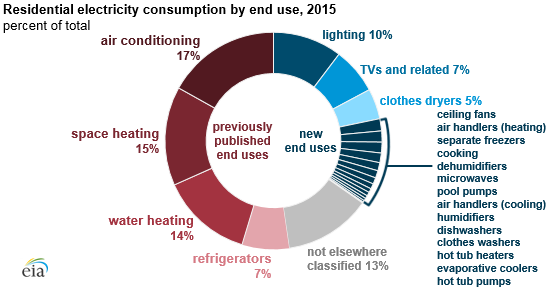
\includegraphics[width=0.9\textwidth]{figures/energy_consumption_in_usa}
    \caption{Residential energy consumption structure in United States, 2015}
\end{figure}

TCLs appear to be excellent candidates candidates for participating in DR programs for at least three reasons:

\begin{enumerate}
    \item Insensitivity to short-term offs. 
    \item Descriptability by Markov Decision Processes
    \item Availability in the majority of residential and commercial premises. 
    \item A big share of consumed energy.
\end{enumerate}
